\begin{minipage}{0.60\textwidth}
    \begin{figure}[h]
    \centering
    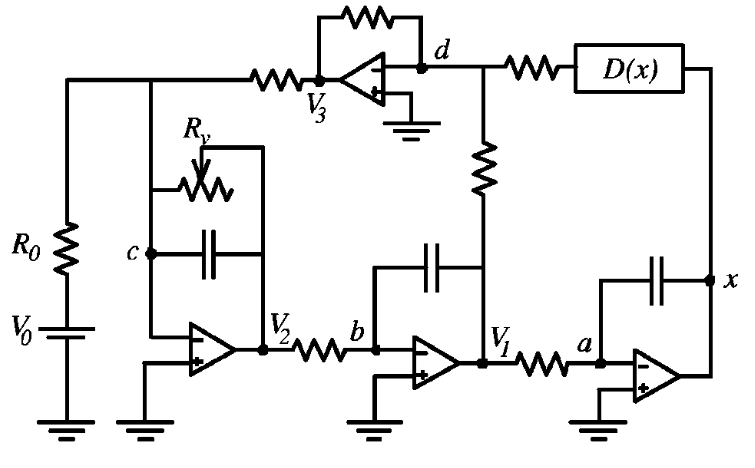
\includegraphics[width=1\textwidth]{images/e_chaotic_circuit.png}
    \caption{Schematic diagram of the circuit used.}
    %\label{fig:}
\end{figure}
\end{minipage}
\hfill
\begin{minipage}{0.35\textwidth}
    \begin{align*}
        &V_1 = - R C \frac{d x}{d t} = - \dot{x} \\
        &V_2 = - R C \frac{d V_1}{d t} = \ddot{x} \\
        &V_3 = - V_1 - D(x)
    \end{align*}
\end{minipage}
\begin{equation}
        \dddot{x} = - \left(\frac{R}{R_v}\right) \ddot{x} - \dot{x} + D(x) - \left(\frac{R}{R_0}\right)V_0.
\end{equation}
